% !TeX spellcheck = en_US
\section{Evaluation}
\label{sec:530_evaluation}
In this section, the performance of the novel \ac{MBS} \ac{LiViU} is evaluated using a prototypical evaluation in two different, realistic streaming situations.
The first streaming situation analyzes the remote streaming case over cellular networks, whereas the second performs an analysis of in situ streaming.
\subsection{Evaluation Setup}
The evaluation consists of different runs repeated under similar conditions.
The experiments are realized using 13 different devices from different smartphone generations, split into two evaluations: remote and in situ streaming
The mobile devices and network connection settings are shown in Table~\ref{table:530_mobileDevice}.

The evaluation is conducted to assess \ac{LiViU}'s performance regarding goodput, overhead, duplicate messages, join time, and  video stream continuity (\ac{CI}), as described in Section~\ref{sec:520_metrics}.
\begin{table}[h]
	\centering
	\caption{Device setup for evaluating LiViU.}
	\begin{tabular}{l c c c}
		& Scenario &  Count & Network\\ \toprule
		\texttt{LG Nexus 4 (N4)}& Remote & 2 & 3G\\
		\texttt{LG Nexus 5 (N5)}  & Remote & 3	& LTE\\
		\texttt{Samsung Galaxy S6 (S6)}& Remote & 1 & LTE\\
		\texttt{Samsung Galaxy S7 (S7)}& Remote & 1 & LTE\\
		\texttt{OnePlus One (OPO)} &   In situ & 6 & 802.11, LTE \\ 
		\bottomrule
	\end{tabular}
	\label{table:530_mobileDevice}
\end{table} 
\subsubsection{Remote Streaming}
For the remote streaming evaluation, three LG Nexus 5, two LG Nexus 4, one Samsung Galaxy S6, one Galaxy S7 and six OnePlus One are used to assess the performance of \ac{LiViU}.
Video streams are transmitted using the cellular network of Deutsche Telekom in Darmstadt. 
The remote streaming scenario was evaluated at different \ac{PoI}s in Darmstadt: a university building, Herrengarten, and Marktplatz.
In any scenario, the movement is limited to pedestrian speed.
All devices are in the same communication cell and share the bandwidth.
The setup consists of a heterogeneous device set connected to different network types, with varying performance.
Additional traffic by other devices was not considered.
The recording side buffer is set to 50 \unit{MB} to compensate for situations where the recorder captures video faster than the network can transport it.
All devices use synchronized clocks achieved by using \ac{NTP} with a single clock server.

As a streaming end-point, the "streamlet.de" server is hosted in a data center near N\"urnberg, Germany.
Each run lasts for approximately twenty minutes, where the initial five minutes leverage the available throughput of the \ac{LTE} network, and the remaining throughput is shaped on the "streamlet.de" server according to an upload trace of the \ac{MBS} YouNow from 06/27/2015.

The videos are recorded and then encoded into three representations at a resolution of \ac{720p} at 3 \unit{$\frac{MBit}{s}$}, 1.5 \unit{$\frac{MBit}{s}$} and 750 \unit{$\frac{KBit}{s}$} at 30 \unit{\ac{FPS}}. 
The \ac{GoP} length is set to 15 frames. 
Thus, an adaptation could occur every half second.

All experiments are repeated five times.
The focus of the remote streaming evaluation is illustrating the advantages of adaptive video streaming.
\subsubsection{In Situ Streaming}
For evaluating the in situ streaming scenario, OnePlus One devices were used, as the other devices do not allow to establish IEEE 802.11 ad-hoc connections.
The OnePlus One devices allow in ad-hoc mode using the IEEE 802.11b standard with at most 11 $\unit{\frac{MBit}{s}}$ of physical layer bandwidth.
They can reliably stream in ad-hoc mode, without any undesired connection resets.
Six devices were used in a stationary device setup and in a mobile setting.
At any time, exactly one sender is active.
\ac{LiViU} has been tested to support multiple senders in close vicinity, too.
A single limitation can be the capped physical bandwidth of the used \ac{IEEE} 802.11 standard.

Similar conditions as for the remote streaming scenario are used.
If not stated otherwise, the produced video representations are encoded at \ac{480p} at 250 \unit{$\frac{KBit}{s}$}, 500 \unit{$\frac{KBit}{s}$} and 750 \unit{$\frac{KBit}{s}$} at 30 \unit{\ac{FPS}}.
The buffer is configured to store up to $250$ milliseconds of the video. 
It is ensured that video chunks of approximately $100$ milliseconds can be decoded independently. 

All experimental runs are repeated six times with a similar setup, where the in situ streaming is evaluated in a stationary and a mobile setup.
The focus in both setups lies on the evaluation of the network characteristics of the system.
Note, that for the mobile setup the same environmental conditions as in the stationary one cannot be guaranteed.
\paragraph{Stationary Setup}
A stationary setup is chosen consisting of six mobile devices with stable positions and within IEEE 802.11 communication range.
Each evaluation run is performed for 10 minutes. 
Figure~\ref{fig:530_SetupNodes} shows the device setup and intended communication between devices.
The experiments are performed in a closed room so that no valid position information can be retrieved. 
Thus, we manually set the location coordinates in the \ac{OS}.

\begin{figure}[tbh!]
	\centering
	
\includegraphics[width=\linewidth]{gfx/500_MobileUpload/Eval_Stationary_setup}
	\caption{Static topology used for the evaluation of LiViU in the in situ scenario.}
	\label{fig:530_SetupNodes}
\end{figure}
The stationary setup is chosen to conduct a parameter study on both the effect of the streaming bit rate on the effective latency and the influence of an increasing number of devices.
The evaluation is conducted at different bit rates - from 250 \unit{$\frac{KBit}{s}$} over 500 \unit{$\frac{KBit}{s}$} to 750 \unit{$\frac{KBit}{s}$} - to study the effect of bit rate on performance.
Also, the number of devices receiving a stream varies from 1 to 5.
In this second experiment, the bit rate is kept constant at 500 \unit{$\frac{KBit}{s}$}. 
\paragraph{Mobile Setup}
In a mobile setup, the in situ streaming functionality is evaluated in six repetitions of similar movements in a limited area.
In a user study a perfect reproduction of movement patterns, and the environmental conditions, could not be achieved.
The experiments consist of 18 minutes per repetition, which is split into three phases of six minutes each.
During the phases, different mobility patterns are evaluated.
In the first phase the movement of solely the receivers is evaluated, where the sending device holds a central position.
The second phase includes stable positions of the receivers, whereas the sending device is in motion.
In the last phase, all devices are in free motion.
Due to the mobility of the devices, connections can be lost at any phase.
All motion is at pedestrian speeds, thus $\leq 7 \frac{km}{h}$.
A fixed bit rate of 500 \unit{$\frac{KBit}{s}$} is utilized in this scenario.
During this evaluation, locations and movement speeds are calculated using \ac{GPS}.
\begin{figure}[tbh!]
	\centering
	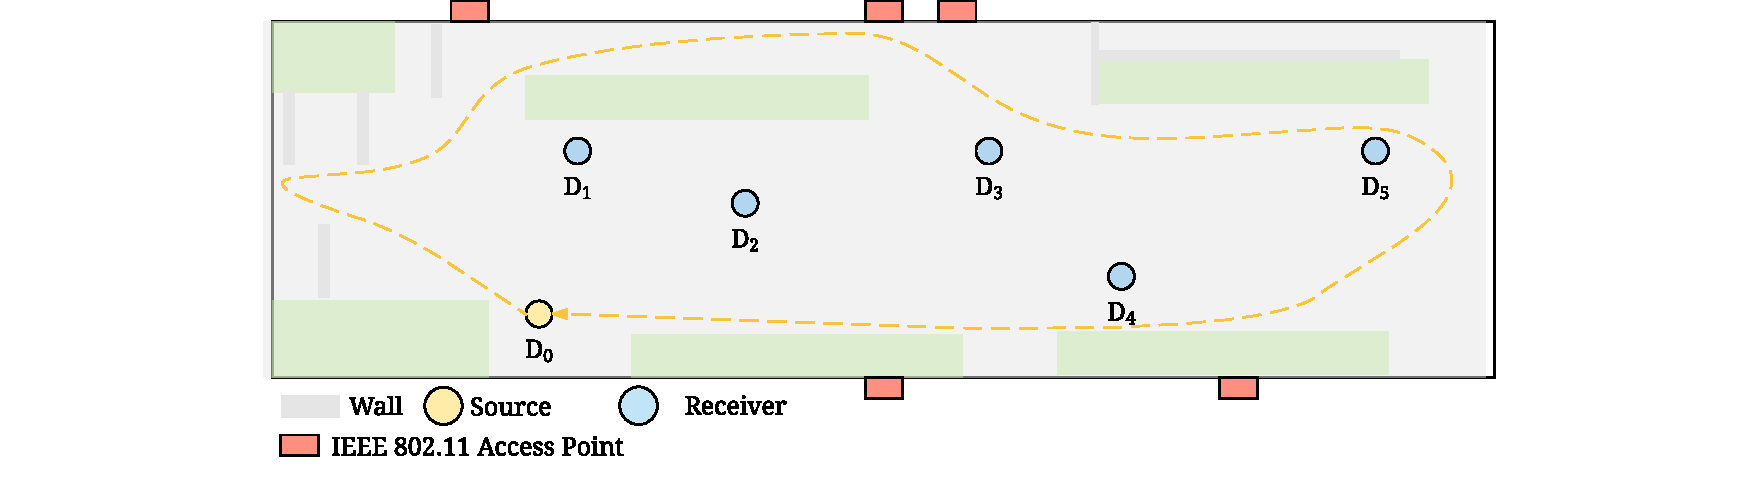
\includegraphics[width=\linewidth]{gfx/500_MobileUpload/EvalMobileScenario_Sender_Moving}
	\caption[Sketch of the evaluation setup for evaluating LiViU's performance]{Sketch of the evaluation setup for evaluating LiViU's performance considering mobility. Figure shows phase 2 of the evaluation in which the sending device is in motion.}
	\label{fig:530_MobileScenario}
\end{figure}
Figure~\ref{fig:530_MobileScenario} depicts an overview of the evaluation space for the mobile setting and depicts the second phase of the described scenario, in which the sender continuously moves.
It indicates that potentially disturbing 802.11 access points may limit communication between the devices.
The illustrated access points are not supporting the device-to-device communication, but act as disturbing elements, as their provided networks compete with ad-hoc networks on the physical bandwidth.
Thus, in this realistic setup, access points can lead to increased packet drops or connection losses in the in situ, ad-hoc communication.
\subsection{Performance for Remote Streaming}
The remote streaming scenario is evaluated in cellular networks with the aim to illustrate the advantages of adaptive video streaming concepts in an \ac{MBS}.
To indicate the performance in comparison to other \ac{MBS}s the initial join time, the continuity of a video stream, the goodput, and the overhead of a streaming session are discussed.
\subsubsection{Effect of Content Adaptation on Join Time}
Part of the join time is the preprocessing of the recorded video for transcoding into different representations, the processing of the \ac{LiViU} application, the transmission and the processing on the server.
The delay is measured from capturing a complete video frame until its storage on the remote server.
The focus lies on the discussion of the processing times on the mobile device running \ac{LiViU} as well as the buffer size on the \ac{LiViU} server.
Transmission delays invoked by the cellular network are not discussed in detail, as \ac{LiViU} does not influence them.

\paragraph{Transcoding Adaptive Video Streams}
The transcoding process ensures that the lower bit rate representations are available first, whereas encoding at the highest bit rate lasts longest.
The time between the first and the last representation is available depends on whether recent H.264/AVC encoding hardware is used.
Figure~\ref{fig:530_bitrate_comparison} (a) gives an overview of the difference of leveraging software and hardware encoding.
Whereas for hardware-support (HW) the time difference between the first and the last representation is below a second, the software-based encoding (SW) requires 8.41 times longer to encode all three representations.
Even the hardware encoding needs an average of 0.61 seconds to have a video frame encoded in all three representations, and thus enable the receiving device to perform an adaptation.
Thus, as soon as a video chunk is encoded at the lowest representation, it is transmitted to the server.
A switch to a higher bit rate representation can be performed as soon as throughput conditions are suitable, higher bit rate chunks are available.
Even under good throughput conditions, an initial upload of the lowest bit rate representation is performed to minimize join time.
\begin{figure}
\centering
\subfloat[]{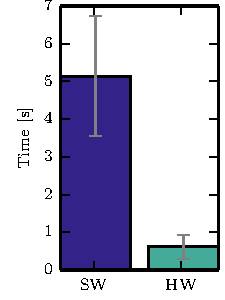
\includegraphics{gfx/500_MobileUpload/LiviuRemoteTranscoding}}
\subfloat[]{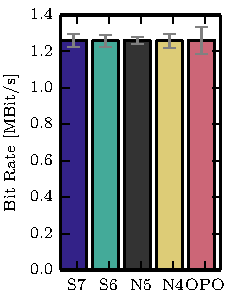
\includegraphics{gfx/500_MobileUpload/LiviuRemoteBitrateToOverhead}}
\subfloat[]{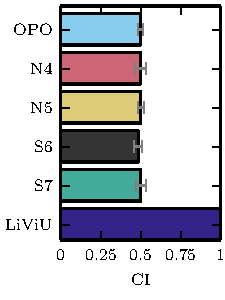
\includegraphics{gfx/500_MobileUpload/LiviuRemoteComparison_AdaptiveNonAdaptive}}
\subfloat[]{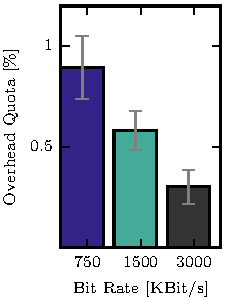
\includegraphics{gfx/500_MobileUpload/LiviuRemoteOverhead}}
\caption[LiViU's performance in the remote streaming scenario]{Overview of the performance when using LiViU for a remote streaming scenario. (a) Transcoding speed for adaptive streaming representations on the video encoding hardware (HW) in comparison with software encoding. (b) Average video bit rate using LiViU in the given scenario. (c) Stalling-free upload using LiViU (CI=1) in comparison with non-adaptive streaming approaches on different devices. (d) Percentage of overhead when using LiViU in comparison to the representation bit rate.}
\label{fig:530_bitrate_comparison}
\end{figure}
\paragraph{Minimal Media Chunk Size}
The size of video chunks being transmitted has an impact on the delay until a stream can be consumed on the receiver side.
At the highest bit rate (3 \unit{$\frac{MBit}{s}$} for remote streaming), a \ac{LiViU} message could transport around 3 milliseconds of video, and at the lowest bit rate representation around 12 milliseconds.
Independent of a segment length the minimal video chunk to be sent should be chosen wisely on the basis of the packet size that can be sent using \ac{UDP}.
There is a trade-off between immediate transmission, encoding efficiency, and minimum bit rate.
When video chunks to be transmitted are smaller than the packet size, the overhead of packet headers will increase detrimental to the goodput.
In the remote streaming scenario, a packet size of up to 950 bytes is chosen.
At a frame rate of 30 \unit{FPS}, this requires that the minimal bit rate of a representation $\geq 228 \unit{\frac{KBit}{s}}$.
Any bit rate lower than $228 \unit{\frac{KBit}{s}}$ would create an unnecessarily high number of messages, which are only partly filled.
The delay is sacrificed to obtain efficient delivery, which keeps the overhead of messages and headers low.
\paragraph{Remaining Components of the Join Time}
Remaining operations of the \ac{LiViU} protocol accounted for 119.78 milliseconds on average, where a single outlier required 692.46 milliseconds.
It could not be clarified what caused this huge increase.
The cellular network caused an additional delay of 79 to 103 milliseconds for \ac{LTE}.
As a result, the delay on the remote streaming side is around 1.7 seconds on average, where a maximum delay of 3.8 seconds has been observed.
Delays related to the serialization of the messages, buffer and main memory operations of the protocols, and  the storage of the stream on the hard disk are not discussed in detail.
\subsubsection{Effect of Content Adaptation on Continuity and Goodput}
The protocol overhead is negligible, as the content adaptation and throughput estimation is solely conducted on the client with local resources.
No coordination is required for the content adaptation, as throughput measurements are offered by an independent monitoring service~\cite{Stohr2014,Stohr2016}.

Under similar conditions, yet with competing devices, the goodput of the adaptive streaming upload achieved 1259.1 \unit{$\frac{KBit}{s}$} on average with a standard deviation of 7.554 \unit{$\frac{KBit}{s}$}.
The differences in repeated runs were mainly caused by uncontrollable environmental changes, such as, e.g., slight variations of the throughput.
They are shown for the five different device types used in the evaluation in Figure~\ref{fig:530_bitrate_comparison} (b).

At the same time, the adaptive video streaming concept on the uploading side of a smart mobile device helps to avoid stalling.
The stall time would have been enormous if no adaptive video streaming approach had been chosen.
The achieved \ac{CI} of 1 is compared with the different devices in Figure~\ref{fig:530_bitrate_comparison} (c).
It can be seen, that when streaming constantly at 3 \unit{$\frac{MBit}{s}$} the \ac{CI} decreases to between 0.4841 and 0.5014 if no adaptive video streaming is used.

The adaptation could achieve consistent streaming without stalling, requiring 9 to 11 adaptations per 10 minutes of video streaming.
All devices streaming in parallel have shown a similar adaptation behavior at similar points in time.
This available throughput drop is caused by the used network trace.
\subsubsection{Overhead}
Per 10 minutes of streaming, the quota of the number of control messages to the total number of messages is below 0.12\% on average, where the size of these messages in comparison to the total traffic generated accounts for only 0.027\%  (see Figure~\ref{fig:530_bitrate_comparison} d). 
This omits the overhead caused by the message headers.
If the lowest bit rate representation (750 \unit{$\frac{KBit}{s}$}) is considered, the total control message traffic as well as the message header, accounts for less than 0.9\% of the total traffic.
% -  -  -  -  -  -  -  -  -  -  -  - -
\subsection{In Situ Streaming Results}
The in situ streaming under challenging conditions, i.e., with mobility, is discussed regarding the bit rates of the streamed video, the effect of mobility on the continuity of the stream as well as the overhead caused by the decentralized organization of the devices.
\subsubsection{Influence of the Representation Bit Rate}
In the stationary setup evaluation, the effect of the video representation's bit rate is evaluated in respect to different performance metrics. 
The influence of the bit rate is given for \ac{CI}, the protocol overhead regarding the number of messages, and the delay.
As a result, the \ac{CI} for this stable condition stays nearly constant, variations below 1\% are observed.
The minimum \ac{CI} still achieves a continuity of above 99\%.
A low \ac{CI} indicates that the protocol is not capable of delivering media chunks in real-time.
Rather hard constraints are given for the recording buffer, which stores approximately 250 milliseconds of the received video stream. 
If packets are lost due to collisions, \ac{LiViU} will request and has to receive the respective video chunks within this window to avoid stalling.
It is obvious from Table~\ref{tab:530_eval_static_results} that the average and maximum delay do not always allow an in-time delivery of the media stream within the receiver's buffer capacity.

\begin{table}[h]
	\centering
	\caption{In situ streaming: Performance of LiViU for varying bit rates.}
	\begin{tabular}{l ccc ccc ccc}%{\textwidth}
		&  \multicolumn{3}{c}{CI [\%]} &   \multicolumn{3}{c}{Delay [ms]} &\multicolumn{3}{c}{Overhead [\%]}  \\
		Bit rate [\unit{$\frac{KBit}{s}$}]& mean & min & $\sigma$ & mean & max & $\sigma$ & mean & max & $\sigma$ \\ \toprule
		\texttt{250 \unit{$\frac{KBit}{s}$}}& 99.87 & 99.74 & 0.041 & 62.9 & 101.54 & 16.64 & 1.33 & 1.361& 0.028\\
		\texttt{500 \unit{$\frac{KBit}{s}$}}& 99.83 & 99.62 & 0.091& 80.13 &117.06 & 21.19 & 1.52 & 1.65 & 0.08 \\
		\texttt{750 \unit{$\frac{KBit}{s}$}}& 99.67 & 99.41 &0.11 & 175.03 &315.86 & 98.42 & 1.79 & 1.91 & 0.07 \\ 
		\bottomrule
	\end{tabular}
	\label{tab:530_eval_static_results}
\end{table} 

The delay increases with the bit rate. 
This indicates throughput limitations of the IEEE 802.11b network, as the maximum effective bandwidth is achieved at a bit rate of 500\unit{$\frac{KBit}{s}$}.
The control overhead quota indicates a slight increase to 1.79\%.
The quota has been chosen to be based on the number of messages and not on the message size, as the control traffic accounts for less than 0.2\% of the total traffic.

This is reliant on the given environmental conditions as well as the number of devices participating in the network.
Especially in the 2.4 \unit{GHz} 802.11 network, a significant increase of in situ devices will limit the bit rate.
The limitation is given by the physical medium and the processing and scheduling capabilities of the devices.
The total join time in the case of in situ streaming is calculated from the availability of a video frame until its playback on the receiver device for a single hop and is 817.83 milliseconds on average ($\sigma = 31.88$ milliseconds). 
In general, \ac{LiViU} offers robust streaming under highly changing video bit rates. 
\subsubsection{Influence of Increasing Interest}
If, during a session, devices join and leave the network, performance metrics may by affected.
Therefore, the topology depicted in Figure~\ref{fig:530_SetupNodes} is set up by joining the devices in a specific order, and leaving the network in the reverse order.
From a single node offering the video stream to the topology depicted in Figure~\ref{fig:530_SetupNodes}, the topology is built up as shown in Figure~\ref{fig:530_SetupNodes_stepBystep}.
Each topology stage is kept for two minutes to achieve stable results.
\begin{figure}[tbh!]
\centering
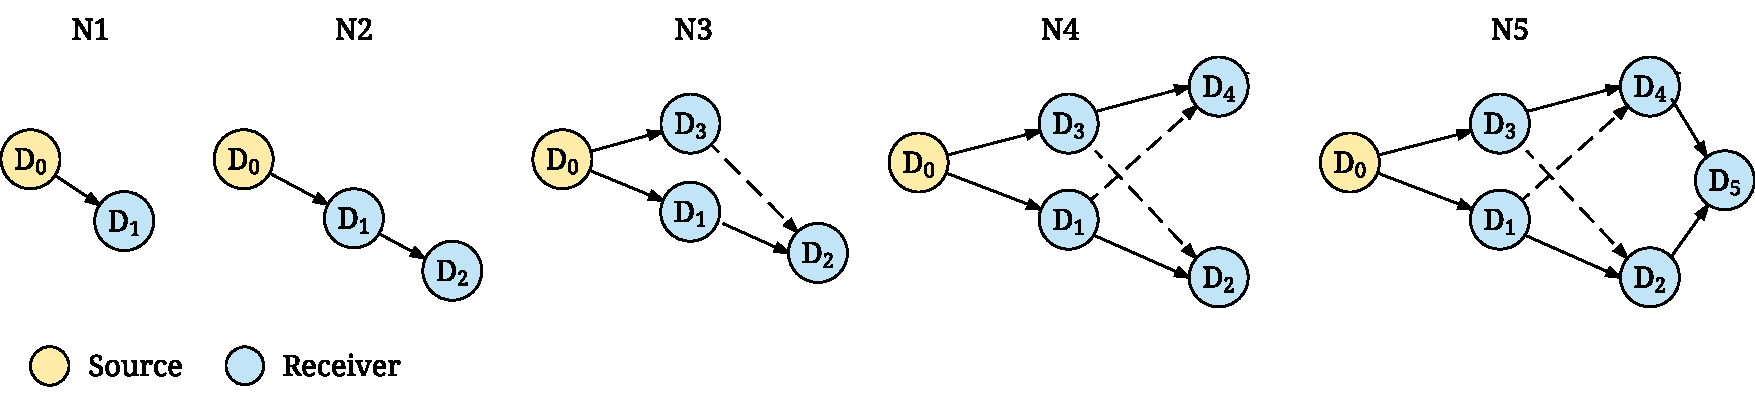
\includegraphics[width=\linewidth]{gfx/500_MobileUpload/Eval_Stationary_setup_Step_by_Step}
\caption{In situ streaming: Performance of LiViU with changing device numbers.}
\label{fig:530_SetupNodes_stepBystep}
\end{figure}
The main finding of the experiments is that LiViU achieves a stable \ac{CI}, which is not reduced until step 3, when $D_2$ can receive video chunks from multiple devices.
The communication of both $D_1$ and $D_3$ leads to an increase of packet losses or error(s) in the packets, and thus a reduced continuity index.
It decreases slightly for $N3$ at an average 99.91\% to $N4$  at 99.81\% and stays stable in $N5$ at 99.83\%, which represents the complete topology.

Similarly, the topology induces a pattern for the control overhead and the quota of redundant chunks received.
For the overhead, the maximum is reached at $N3$ at a control overhead of 1.81\%, and in the remaining rounds it is either stable or it declines.
As the overhead is calculated in relation to the total number of packets, a peak is reached when most devices are in close range and need to coordinate themselves.
Redundant video messages are received when a new device joins the network to quickly retrieve the stream - and if uncoordinated senders in close vicinity to each other do not know of each other as the distribution tree becomes deep, as e.g., for $D_2$, $D_4$ and $D_5$.
Due to the proposed routing in \ac{LiViU} which sends messages based on the distance and bearing between devices, no clear indication is available, which device should deliver video to $D_5$.
As long as the receiver does not unlink from one device, it will send video chunks.
Whereas the redundant video chunk rate increases for $D_5$ up to at a maximum of 48.74\% and in average 23.29\%, the proposed unlinking coordination by the receivers limits to a maximum of 8.2\% of redundant messages.
\subsubsection{Influence of Mobility}
In the second experiment, the mobility of devices (in three phases) is evaluated, consisting of solely receiver mobility, sender mobility only, and a combined evaluation if all devices move.

\ac{LiViU}'s reliability and costs are assessed in environments where devices leave the communication range due to mobility, delays vary, and streaming quality as measured by \ac{CI} degrades.
Also, different \ac{IEEE} 802.11 access points compete with the ad-hoc network established by \ac{LiViU}.

 \begin{table}[h]
 	\centering
 \caption[In situ streaming: Performance in the mobile scenario.]{In situ streaming: Performance in the mobile scenario. Phase 1: Receivers are moving, Phase 2: Sender is moving, and Phase 3: all devices in motion.}
 	\begin{tabular}{l ccc ccc ccc}%{\textwidth}
 		&  \multicolumn{3}{c}{Phase 1} &   \multicolumn{3}{c}{Phase 2} &\multicolumn{3}{c}{Phase 3}  \\
 		\specialcell{Run}& mean & max & min & mean & max & min& mean & max &min \\ \toprule
 		Delay [ms]& 116.57 & 172.71 & 79.8 & 98.86 & 174.26 & 41.35 & 138.56 & 188.29 & 94.77\\
 		CI [ms]& 97.66 & 99.82 & 94.15 & 98.81 & 99.9 & 95.65 & 96.74 & 99.32 & 91.25\\ 
 		%Duplicates [\%]& 22.85 & 37.75 & 13.22& 21.68 & 45.7 & 0 & 7.94 & 35.74  & 0\\ 
 		CO [\%]	& 4.03 & 5.54 & 1.81 & 2.99 & 7.67 & 0.93 & 6.05 & 11.49 & 2.34 \\ 
 		Speed Receivers [\unit{$\frac{m}{s^2}$}]& 0.811 & 0.927 & 0.599& 0 & 0 & 0 & 0.917 & 1.038 & 0.735 \\ 
 		Speed Sender [\unit{$\frac{m}{s^2}$}]& 0 & 0 &0 & 0.974 & 1.03 & 0.924& 0.959& 1.04& 0.895 \\ 
 		\bottomrule
 	\end{tabular}
 	\label{tab:530_mobility_scenario_eval}
 \end{table} 

The results, including the speeds of the devices, are shown in Table~\ref{tab:530_mobility_scenario_eval}.
Mobility has a significant impact on the \ac{CI}, which in the case of all devices in motion drops to a minimum of 91.25\%, where the average in the session is 96.74\%.
Still, in spite of potential connection losses and re-routing requirements in the scenario, it is ensured that $\geq 90\%$ of the stream is received and played back in time.
The delay from recording until playback is $< 650$ milliseconds and thus comparably faster than infrastructure-based approaches with delays around 1 second~\cite{Dezfuli2013}.
The increased control overhead (especially in phase 3 where all nodes are moving) depicts that the required coordination leads to more messages being exchanged.

In the mobile scenario, the likelihood of redundant delivery of video messages from different senders to the same receiver is high.
The receiving devices can determine, which devices shall stop sending using unlink messages.
This mechanism ensures that the duplicate chunk ratio reduced to in average 1.9\% at a maximum of 6.03\%.
\subsection{Discussion}
The proposed \ac{MBS} \ac{LiViU} achieves efficient streaming both to remote and close-by devices.
For remote receivers, the benefits include reliable streaming while coping with rapidly changing throughput conditions, a quick connection setup, and adaptation to different scenarios. The in situ streaming achieves minimal delay between devices while independently organizing the streaming topology at the cost of redundant messages.
The evaluation shows that reliable streaming can be achieved despite mobility.

In comparison to other work~\cite{Dezfuli2013,Niraula2009}, \ac{LiViU} achieves a lower delay with considerably less overhead.
Furthermore, Niraula et al. show for mobile scenarios that stall-free streaming is possible at a bit rate of 128 \unit{$\frac{KBit}{s}$}, which is lower than the bit rate that \ac{LiViU} supports (500 to 750 \unit{$\frac{KBit}{s}$}).
Furthermore, adaptive video streaming is supported by \ac{LiViU} on the mobile device.
In contrast to the work of Seo et al.~\cite{Seo2012}, the proposed system achieves a reduced delay with similar video recording settings, but in cellular networks.
Whereas, the proposed \ac{LiViU} system achieves a reliable streaming of \ac{720p} content in cellular networks without any control of the network, Seo. et al.~\cite{Seo2012} ran their experiments in private \ac{IEEE} 802.11 networks without competing traffic.
Thus, for high resolutions of up to \ac{720p} and non-recent devices, live streaming was not possible.
In contrast to their approach, \ac{LiViU} achieves in-parallel encoding of three \ac{720p} videos in real-time, as well as their delivery to remote servers and close-by devices.
The availability of different video representations allows adaptation according to the network conditions smoothly.
It can be concluded that \ac{LiViU} achieves reliable video streaming in the different streaming scenarios.